\documentclass{article}
\usepackage[utf8]{inputenc}
\usepackage{hyperref}

\title{Übung 4}
\author{Laurenz Weixlbaumer, 11804751}
\date{November 2018}

\renewcommand\thesubsection{(\alph{subsection})}

\usepackage{enumitem}
\usepackage{mathtools}

\begin{document}

\maketitle

\stepcounter{section}\stepcounter{section}
\section{Multiplikation im Zweierkomplement}

\begin{enumerate}[label=(\alph*)]

\item Paralleler 2-Bit Multiplizierer.

\begin{figure}[h]
\begin{center}
    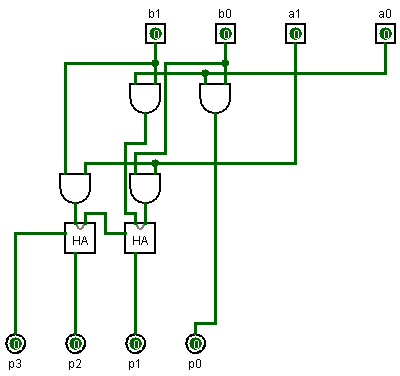
\includegraphics[width=10cm]{multiplier_prl_circuit.png}
\end{center}
\end{figure}

\clearpage

\item Berechnung des Produkts von $01_2$ und $11_2$, die Pegel an den Ein- und Ausgängen, Addierern und Gattern sind farblich hervorgehoben.

\begin{figure}[h]
\begin{center}
    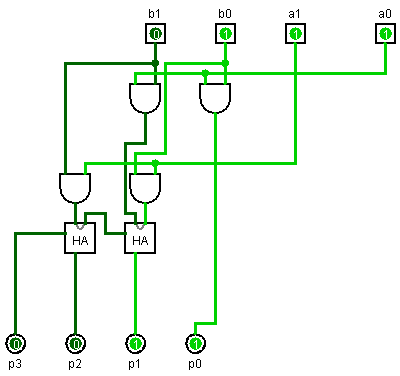
\includegraphics[width=10cm]{multiplier_prl_circuit_marked.png}
\end{center}
\end{figure}

\end{enumerate}

\end{document}
